\chapter{Ácidos, bases y pH}\label{ch:g9:acids-bases-ph}

En un estante de la cocina hay un limón, una botella de vinagre, una
pastilla de jabón y una caja de bicarbonato; debajo del fregadero, un
bote de desatascador con una etiqueta de advertencia negra y roja.
Algunos tienen un sabor ácido, otros resultan resbaladizos al tacto,
otros pueden quemar la piel. Una sola escala, numerada de 0 a 14, los
ordena a todos, y la misma escala se usa para las piscinas, la tierra
del jardín, la sangre y los océanos.

\begin{recall}
Los \omterm{def:g9:ions:ion}{iones} son \omterm{def:g7:atoms-and-molecules:atom}{átomos} o grupos de \omterm{def:g7:atoms-and-molecules:atom}{átomos} con carga; un \omterm{def:g9:ions:ion}{catión} como
\ce{Na+} es positivo, y un \omterm{def:g9:ions:ion}{anión} como \ce{Cl-} o \ce{OH-}, negativo.
Las disoluciones iónicas contienen \omterm{def:g9:ions:ion}{iones}, marcados con (aq), que se
mueven libremente (\cref{ch:g9:ions}).
\end{recall}

\begin{omfigure}
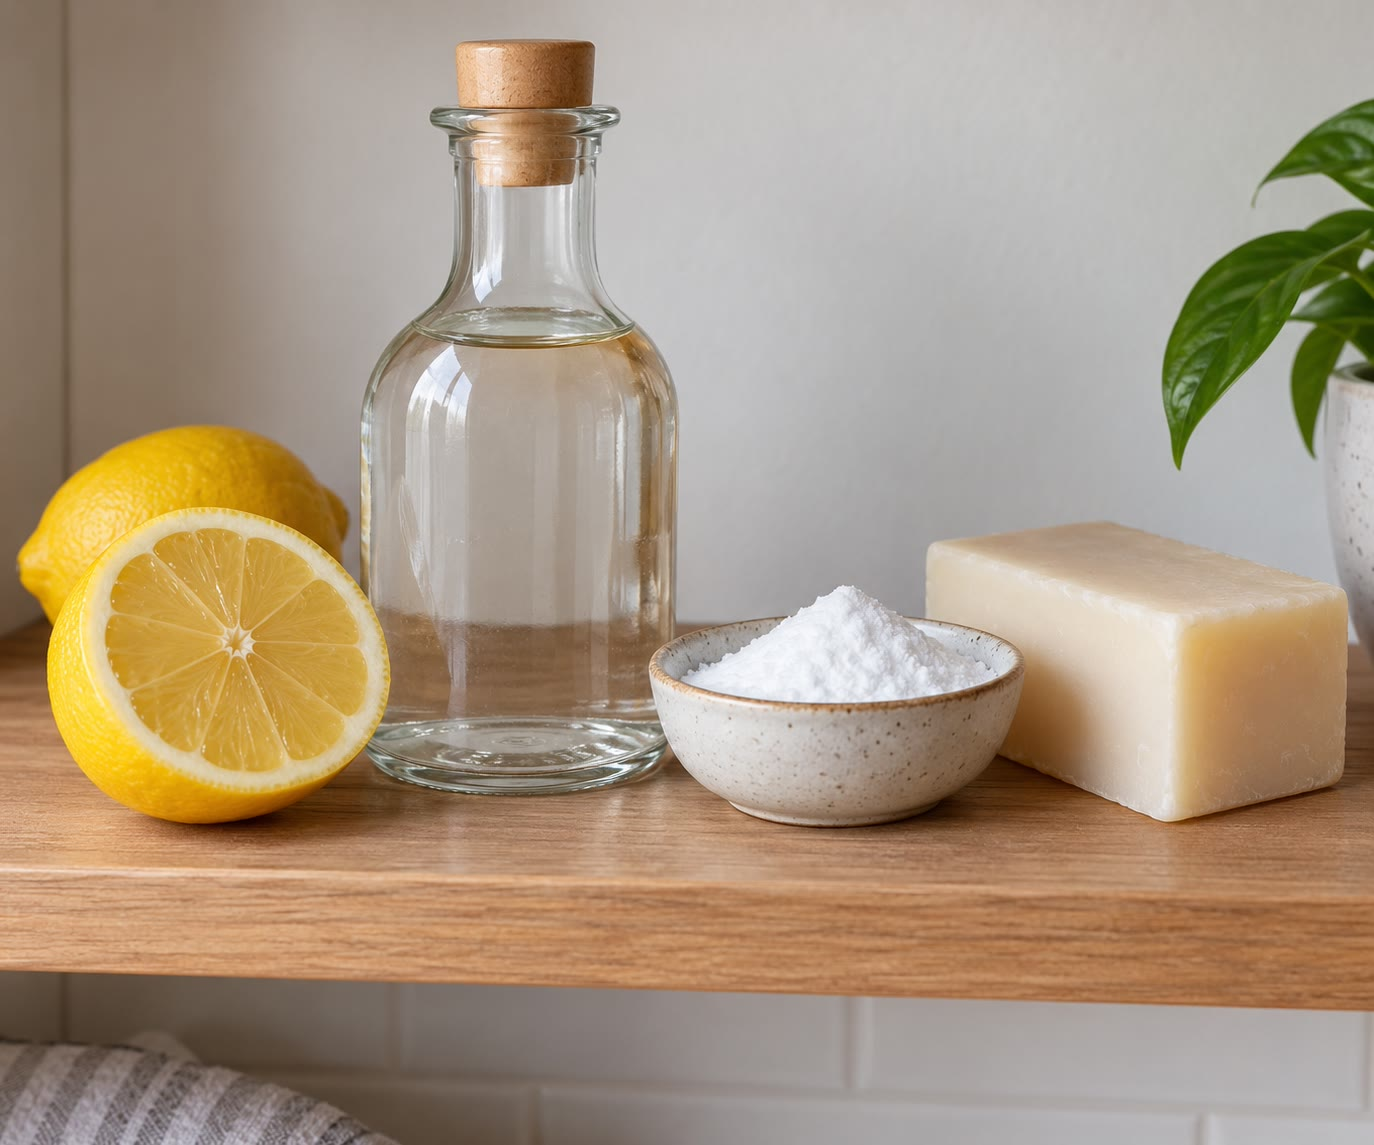
\includegraphics[width=0.55\linewidth]{images/book1/ai/g9-kitchen-shelf.jpg}

{\small Limón, vinagre, jabón y bicarbonato: ácidos y bases en la
cocina.}
\end{omfigure}

\section{Disoluciones ácidas, básicas y neutras}

\begin{definition}[Disoluciones ácidas, básicas y neutras]\label{def:g9:acids-bases-ph:acidic}
Toda \omterm{def:g6:solutions-and-solubility:solute}{disolución acuosa} contiene \omterm{def:g9:ions:ion}{iones} hidrógeno \ce{H+(aq)} e \omterm{def:g9:ions:ion}{iones}
hidróxido \ce{OH-(aq)}. Una disolución es una
\emph{disolución ácida}\index{disolucion acida@disolución ácida}
cuando contiene más \omterm{def:g9:ions:ion}{iones} \ce{H+} que \omterm{def:g9:ions:ion}{iones} \ce{OH-}, una
\emph{disolución básica}\index{disolucion basica@disolución básica} cuando contiene más
\omterm{def:g9:ions:ion}{iones} \ce{OH-} que \omterm{def:g9:ions:ion}{iones} \ce{H+}, y una \emph{disolución
neutra}\index{disolucion neutra@disolución neutra} cuando contiene tantos de unos como de
otros.
\end{definition}

\begin{example}[Tres disoluciones]\label{ex:g9:acids-bases-ph:three}
El ácido clorhídrico es una \omterm{def:g9:acids-bases-ph:acidic}{disolución ácida}: contiene \omterm{def:g9:ions:ion}{iones}
\ce{H+(aq)} y \ce{Cl-(aq)}, con muy pocos \ce{OH-}. Una disolución de
hidróxido de sodio es básica: \ce{Na+(aq)} y \ce{OH-(aq)}, con muy pocos
\ce{H+}. El agua pura y el agua salada son neutras.
\end{example}

\section{La escala de pH}

\begin{definition}[pH]\label{def:g9:acids-bases-ph:ph}
El \emph{pH}\index{pH} de una \omterm{def:g6:solutions-and-solubility:solute}{disolución acuosa} es un número, por lo
general entre 0 y 14, que indica lo ácida o básica que es: a
\qty{25}{\celsius}, una \omterm{def:g9:acids-bases-ph:acidic}{disolución neutra} tiene pH 7, una \omterm{def:g9:acids-bases-ph:acidic}{disolución
ácida} un pH inferior a 7 y una \omterm{def:g9:acids-bases-ph:acidic}{disolución básica} un pH superior a 7.
Cuantos más \omterm{def:g9:ions:ion}{iones} \ce{H+} contiene una disolución, más bajo es su pH.
\end{definition}

\begin{omfigure}
\begin{tikzpicture}[font=\small, x=0.95cm]
  \foreach \k in {0,...,13} {
    \pgfmathtruncatemacro\rr{2.2*max(0,100-14.3*\k)+30}
    \pgfmathtruncatemacro\gg{1.8*(\k<7 ? 30+10*\k : 100-8*(\k-7))+40}
    \pgfmathtruncatemacro\bb{2.2*max(0,14.3*(\k-6))+30}
    \definecolor{phc}{RGB}{\rr,\gg,\bb}
    \fill[phc] (\k,0) rectangle ++(1,0.6);
  }
  \foreach \k in {0,...,14} \node[anchor=north, font=\footnotesize] at (\k,-0.02) {\k};
  \draw[black!60] (0,0) rectangle (14,0.6);
  \node[anchor=south] at (3.5,0.65) {ácida};
  \node[anchor=south] at (7,0.65) {neutra};
  \node[anchor=south] at (10.5,0.65) {básica};
  % ledger: ph:HCl-1M, ph:gastric, ph:lime, ph:wine, ph:coffee, ph:pure-water, ph:seawater, ph:milk-magnesia, ph:ammonia, ph:NaOH-1M
  \foreach \x/\lab/\lev/\anc in {0/{ácido\\ clorhídrico (1 M)}/1/north, 1.5/{jugos\\ gástricos}/3/north east,
      2/{zumo\\ de lima}/2/north west, 3.5/{vino}/1/north, 5/{café}/2/north, 7/{agua\\ pura}/3/north,
      8.1/{agua\\ de mar}/1/north, 10.5/{leche de\\ magnesia}/3/north, 12/{amoniaco\\ doméstico}/1/north,
      14/{hidróxido de sodio\\ (1 M)}/2/north east} {
    \draw[black!55] (\x,-0.45) -- (\x,-0.45-0.8*\lev);
    \node[anchor=\anc, font=\footnotesize, align=center, inner sep=2pt] at (\x,-0.45-0.8*\lev) {\lab};
  }
\end{tikzpicture}

{\small La escala de \omterm{def:g9:acids-bases-ph:ph}{pH}, con el \omterm{def:g9:acids-bases-ph:ph}{pH} de algunas disoluciones corrientes.}
\end{omfigure}

\begin{definition}[Papel indicador y pHmetro]\label{def:g9:acids-bases-ph:ph-paper}
El \emph{papel indicador}\index{papel indicador} es una tira de papel
impregnada de una \omterm{def:g6:pure-substances-and-mixtures:mixture}{mezcla} de colorantes que toma un color distinto para
cada \omterm{def:g9:acids-bases-ph:ph}{pH}; se pone en ella una gota de la disolución y se compara el
color con una escala impresa en la caja. Un
\emph{pHmetro}\index{pHmetro} mide el \omterm{def:g9:acids-bases-ph:ph}{pH} con una sonda de vidrio
sumergida en la disolución y lo muestra como un número, con uno o dos
decimales.
\end{definition}

\begin{method}[Medir un pH con papel indicador]\label{met:g9:acids-bases-ph:paper}
\begin{enumerate}
  \item Poner una tira corta de \omterm{def:g9:acids-bases-ph:ph-paper}{papel indicador} en un recipiente limpio
        y seco.
  \item Con una varilla de vidrio limpia, tocar la tira con una gota de
        la disolución (no meter nunca la tira en el frasco).
  \item Comparar enseguida el color con la escala y leer el \omterm{def:g9:acids-bases-ph:ph}{pH}, por lo
        general al número entero más próximo.
\end{enumerate}
\end{method}

\begin{omfigure}
\begin{tikzpicture}[font=\small, scale=1.2]
  \pic[transform shape] at (0,0) {stirrer};
  \pic[transform shape] at (0,0.05) {beaker={0.55}{omWater!80}};
  \pic[transform shape] at (0.25,0.35) {probe};
  \pic[transform shape] at (2.6,3.4) {meter={pH}};
  \draw[black!70, line width=0.6pt] (0.25,3.45) .. controls (0.3,4.3) and (2.2,4.4)
    .. (2.2,2.95);
  \draw[<-, omProp, thick] (0.4,1.0) -- (2.0,1.3) node[right, text=black] {sonda de vidrio};
  \draw[<-, omProp, thick] (3.35,3.4) -- (4.0,3.4) node[right, text=black] {pHmetro};
  \draw[<-, omProp, thick] (-0.6,0.6) -- (-1.6,0.9) node[left, text=black] {disolución};
\end{tikzpicture}

{\small Medida de un \omterm{def:g9:acids-bases-ph:ph}{pH} con un \omterm{def:g9:acids-bases-ph:ph-paper}{pHmetro}: la sonda de vidrio está
sumergida en la disolución, que se agita suavemente.}
\end{omfigure}

\section{Diluir un ácido}

\begin{proposition}[Diluir acerca el pH a 7]\label{prop:g9:acids-bases-ph:dilution}
Al añadir agua a una \omterm{def:g9:acids-bases-ph:acidic}{disolución ácida}, sus \omterm{def:g9:ions:ion}{iones} \ce{H+} se reparten en
un volumen mayor: el \omterm{def:g9:acids-bases-ph:ph}{pH} sube, hacia 7, pero nunca lo supera. Para un
ácido como el ácido clorhídrico, diluir diez veces sube el \omterm{def:g9:acids-bases-ph:ph}{pH} en una
unidad, más o menos: un volumen de ácido de \omterm{def:g9:acids-bases-ph:ph}{pH} 2 más nueve volúmenes de
agua dan una disolución de \omterm{def:g9:acids-bases-ph:ph}{pH} 3. Del mismo modo, diluir una \omterm{def:g9:acids-bases-ph:acidic}{disolución
básica} hace bajar su \omterm{def:g9:acids-bases-ph:ph}{pH} hacia 7.
\end{proposition}

\begin{omfigure}
\begin{tikzpicture}[font=\small, scale=1.05]
  \foreach \k/\ph/\cc in {0/2/red!38!omWater,1/3/red!24!omWater,2/4/red!12!omWater} {
    \pic[transform shape] at (\k*4.4,0) {beaker={0.55}{\cc}};
    \node[anchor=north, align=center] at (\k*4.4,-0.15) {pH \ph};
  }
  \foreach \k in {0,1} \draw[->, thick, omProp] (\k*4.4+1.1,1.0) -- (\k*4.4+3.3,1.0)
    node[midway, above, text=black, font=\footnotesize, align=center]
    {10 mL + 90 mL\\ de agua};
\end{tikzpicture}

{\small Se diluye un ácido diez veces, y luego otras diez: el \omterm{def:g9:acids-bases-ph:ph}{pH} pasa de
2 a 3 y a 4 (cada vaso es una décima parte de la disolución anterior
completada con agua).}
\end{omfigure}

\begin{inthelab}[Diluir un ácido]
Para diluir un ácido, el profesor vierte siempre el ácido despacio sobre
el agua, nunca el agua sobre el ácido: la \omterm{def:g6:pure-substances-and-mixtures:mixture}{mezcla} desprende calor, y el
agua vertida sobre un ácido concentrado puede hervir de golpe y
salpicar ácido fuera del recipiente.
\end{inthelab}

\section{Ácidos y bases de todos los días}

\begin{proposition}[Ácidos y bases a nuestro alrededor]\label{prop:g9:acids-bases-ph:everyday}
Ácidos: el zumo de limón y de lima, el vinagre, el vino, los refrescos
con gas, el café, los jugos gástricos del estómago. Básicos: el agua de
mar (ligeramente), el bicarbonato disuelto en agua, el jabón, la leche
de magnesia (un remedio contra la acidez de estómago), el amoniaco
doméstico, la lejía, el desatascador (muy fuertemente).
\end{proposition}

\begin{example}[El pH del océano]\label{ex:g9:acids-bases-ph:ocean}
% ledger: ph:seawater, ph:ocean-drop
El \omterm{def:g9:acids-bases-ph:ph}{pH} medio del océano es de alrededor de 8.1: ligeramente básico. Desde
el comienzo de la era industrial, el dióxido de carbono que se \omterm{def:g2:mixing-and-dissolving:dissolve}{disuelve}
desde el \omterm{def:g4:air-a-mixture-of-gases:air}{aire} ha hecho bajar el \omterm{def:g9:acids-bases-ph:ph}{pH} de las aguas superficiales en unas
0.1 unidades: los océanos se van volviendo poco a poco menos básicos, lo
que perjudica a los moluscos y a los corales.
\end{example}

\begin{omfigure}
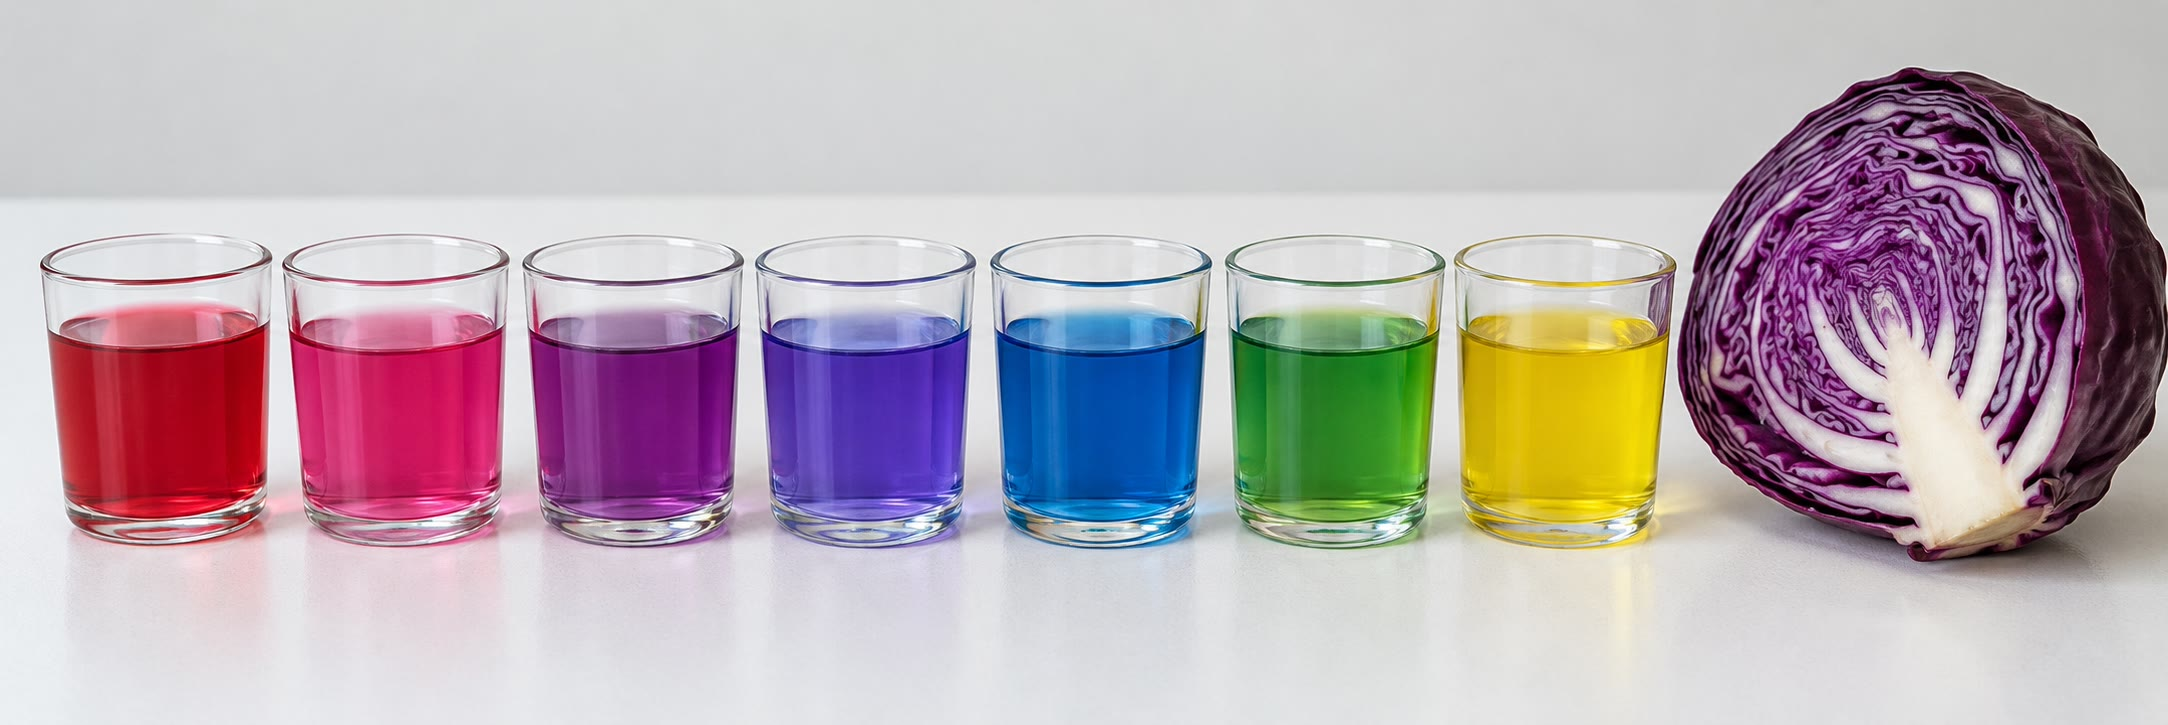
\includegraphics[width=0.55\linewidth]{images/book1/ai/g9-red-cabbage.jpg}

{\small El jugo de lombarda, preparado por un profesor, cambia de color
con el \omterm{def:g9:acids-bases-ph:ph}{pH}: rojo en los ácidos, violeta cerca de la neutralidad, y azul,
verde y luego amarillo en disoluciones cada vez más básicas.}
\end{omfigure}

\section{Seguridad con los productos corrosivos}

\begin{safety}{\ghs[0.85cm]{GHS05}\ghs[0.85cm]{GHS07}}
% ledger: ghs:HCl, ghs:NaOH
El ácido clorhídrico concentrado y el hidróxido de sodio (la base de los
desatascadores) llevan el pictograma de corrosión GHS05: provocan
quemaduras graves en la piel y en los ojos y atacan los metales. GHS07:
irritante. Gafas y guantes; una salpicadura se enjuaga enseguida con
mucha agua.
\end{safety}

\begin{remark}[No mezclar nunca productos de limpieza]\label{rem:g9:acids-bases-ph:mix}
Los productos ácidos y básicos reaccionan entre sí, a veces
violentamente, y algunas \omterm{def:g6:pure-substances-and-mixtures:mixture}{mezclas} liberan gases tóxicos: la lejía
\omterm{def:g2:mixing-and-dissolving:mix}{mezclada} con un desincrustante ácido desprende cloro. Los productos de
limpieza no se \omterm{def:g2:mixing-and-dissolving:mix}{mezclan} nunca.
\end{remark}

\section{Ejercicios}

\begin{exercise}[$\star$]\label{exo:g9:acids-bases-ph:1}
¿Ácida, básica o neutra? Una disolución de \omterm{def:g9:acids-bases-ph:ph}{pH} 3, una de \omterm{def:g9:acids-bases-ph:ph}{pH} 7, una de
\omterm{def:g9:acids-bases-ph:ph}{pH} 11.
\end{exercise}

\begin{exercise}[$\star$]\label{exo:g9:acids-bases-ph:2}
¿Qué \omterm{def:g9:ions:ion}{iones} son más numerosos en una \omterm{def:g9:acids-bases-ph:acidic}{disolución ácida}? ¿Y en una básica?
\end{exercise}

\begin{exercise}[$\star$]\label{exo:g9:acids-bases-ph:3}
Con la escala de \omterm{def:g9:acids-bases-ph:ph}{pH} de este capítulo, ordena de la más ácida a la más
básica: el café, el agua de mar, el zumo de lima, el amoniaco doméstico,
el agua pura.
\end{exercise}

\begin{exercise}[$\star$]\label{exo:g9:acids-bases-ph:4}
Describe cómo se mide el \omterm{def:g9:acids-bases-ph:ph}{pH} de una disolución con \omterm{def:g9:acids-bases-ph:ph-paper}{papel indicador}.
\end{exercise}

\begin{exercise}[$\star\star$]\label{exo:g9:acids-bases-ph:5}
Una disolución de \omterm{def:g9:acids-bases-ph:ph}{pH} 4 se diluye diez veces con agua. ¿Cuál es,
aproximadamente, su nuevo \omterm{def:g9:acids-bases-ph:ph}{pH}? ¿Y si se diluye cien veces?
\end{exercise}

\begin{exercise}[$\star\star$]\label{exo:g9:acids-bases-ph:6}
¿Puede una \omterm{def:g9:acids-bases-ph:acidic}{disolución ácida} volverse básica añadiéndole agua? Explícalo.
\end{exercise}

\begin{exercise}[$\star\star$]\label{exo:g9:acids-bases-ph:7}
¿Por qué hay que verter el ácido sobre el agua, y no al revés?
\end{exercise}

\begin{exercise}[$\star\star$]\label{exo:g9:acids-bases-ph:8}
Un frasco lleva el pictograma GHS05. ¿Qué significa? Da dos
precauciones.
\end{exercise}

\begin{exercise}[$\star\star$]\label{exo:g9:acids-bases-ph:9}
¿Cuántas diluciones por diez hacen falta para llevar un ácido de \omterm{def:g9:acids-bases-ph:ph}{pH} 1 a
\omterm{def:g9:acids-bases-ph:ph}{pH} 4? ¿Qué dilución total es esa?
\end{exercise}

\begin{exercise}[$\star\star$]\label{exo:g9:acids-bases-ph:10}
La leche de magnesia se toma contra la acidez de estómago. Con la escala
de \omterm{def:g9:acids-bases-ph:ph}{pH}, explica por qué.
\end{exercise}

\begin{exercise}[$\star\star\star$]\label{exo:g9:acids-bases-ph:11}
El \omterm{def:g9:acids-bases-ph:ph}{pH} del océano ha bajado unas 0.1 unidades desde la era industrial.
¿Es ácido hoy el océano? ¿En qué sentido evoluciona, y por qué?
\end{exercise}

\begin{exercise}[$\star\star\star$]\label{exo:g9:acids-bases-ph:12}
Un alumno mide el \omterm{def:g9:acids-bases-ph:ph}{pH} del mismo vinagre con \omterm{def:g9:acids-bases-ph:ph-paper}{papel indicador} (3) y con un
\omterm{def:g9:acids-bases-ph:ph-paper}{pHmetro} (2.6). Explica por qué difieren los dos resultados y cuál es más
preciso.
\end{exercise}

\section{Problema: El ácido derramado}

\begin{problem}[{Problema de fin de semana --- un litro de ácido
derramado en un fregadero de laboratorio, y por qué diluirlo no es la
solución}]
\label{pb:g9:acids-bases-ph:1}
Un frasco que contiene \qty{1}{L} de ácido clorhídrico diluido, de
\omterm{def:g9:acids-bases-ph:ph}{pH} 2, se rompe en un fregadero de laboratorio. El desagüe no debe
recibir ninguna disolución de \omterm{def:g9:acids-bases-ph:ph}{pH} inferior a 5. Toma la regla de este
capítulo: para este ácido, cada dilución por diez sube el \omterm{def:g9:acids-bases-ph:ph}{pH} en una
unidad.

\medskip
\noindent\textbf{Parte I --- El ácido.}
\begin{enumerate}
  \item ¿La disolución es ácida, neutra o básica? ¿Qué \omterm{def:g9:ions:ion}{iones} contiene en
        mayor cantidad?
  \item ¿Qué pictograma debería llevar el frasco, y por qué?
  \item El profesor mide el \omterm{def:g9:acids-bases-ph:ph}{pH} con un \omterm{def:g9:acids-bases-ph:ph-paper}{pHmetro} en lugar de con \omterm{def:g9:acids-bases-ph:ph-paper}{papel
        indicador}. Da una ventaja.
  \item ¿Cuántas veces más \omterm{def:g9:ions:ion}{iones} \ce{H+} hay en un litro de \omterm{def:g9:acids-bases-ph:ph}{pH} 2 que en
        un litro de \omterm{def:g9:acids-bases-ph:ph}{pH} 3 del mismo ácido?
\end{enumerate}

\medskip
\noindent\textbf{Parte II --- Diluir.}
\begin{enumerate}[resume]
  \item ¿Qué volumen de disolución se obtiene al diluir diez veces el
        litro de ácido? ¿Cuál es su \omterm{def:g9:acids-bases-ph:ph}{pH}?
  \item ¿Cuántas diluciones por diez hacen falta para llegar a \omterm{def:g9:acids-bases-ph:ph}{pH} 5?
  \item ¿Qué volumen total de disolución se obtendría?
  \item ¿Podría alguna cantidad de agua volver básica la disolución?
        Explícalo.
\end{enumerate}

\medskip
\noindent\textbf{Parte III --- Una manera mejor.}
En su lugar, el profesor añade poco a poco una disolución de una base
hasta que el \omterm{def:g9:acids-bases-ph:ph-paper}{papel indicador} marca 7: los \omterm{def:g9:ions:ion}{iones} \ce{H+} del ácido
reaccionan con los \omterm{def:g9:ions:ion}{iones} \ce{OH-} de la base.
\begin{enumerate}[resume]
  \item Escribe la ecuación de la reacción entre los \omterm{def:g9:ions:ion}{iones} \ce{H+} y
        \ce{OH-}.
  \item ¿Por qué es mejor esto que diluir?
  \item Nombra un producto básico de uso diario que podría servir en una
        cocina para limpiar un pequeño derrame de vinagre.
  \item Calcula el volumen de agua que habría que añadir al litro de
        ácido para llevarlo a \omterm{def:g9:acids-bases-ph:ph}{pH} 5.
\end{enumerate}
\end{problem}
